\documentclass{article}
\usepackage[utf8]{inputenc}
\usepackage{authblk}
\usepackage{url}

\title{Bit Sensitvity of Primitive Hash Functions}
\author{Joshua Weinstein}
\affil{Splunk Inc}
\date{May 2020}

\usepackage{natbib}
\usepackage{graphicx}
\usepackage{amsmath}
\usepackage{amsfonts}
\usepackage{amsthm}
\usepackage{amssymb}
\usepackage{pgfplots}
\pgfplotsset{width=10cm,compat=1.9}
\newtheorem{definition}{Definition}[subsection]
\newtheorem{theorem}{Theorem}[subsection]

\def\Qop{\operatornamewithlimits{%
  \mathchoice{\vcenter{\hbox{\huge Q}}}
             {\vcenter{\hbox{\Large Q}}}
             {\mathrm{Q}}
             {\mathrm{Q}}}}

\begin{document}

\maketitle

\begin{abstract}
Can performance optimized hash functions be used as checksum functions? Common data structures like hash tables depend on hash functions to provide high performance and throughput. The hash functions used in such data structures are nearly all primitive. Primitive hash functions use one repeated statement of operations over the bytes of some input to produce a digest, as opposed to many rounds of iteration in cryptographic hash functions. This work seeks to test the bit sensitivity of primitive hash functions in regards to their digests. Primitive operations from popular hash functions, among others, are tested for absolute bit flips and degrees of bit sensitivity. Results are discussed and evaluated for the potential use of primitive hash operations in designing data integrity check-sums. 
\end{abstract}

\section{Introduction}
A primitive hash function (PMF) generates digests with fast performance, often used in map-oriented data structures. Several widely used implementations of hash maps, like Dictionaries\citep{PythonDJB2} in the Python programming language, opt for the use of a primitive hash function, such as DJB2. These types of hash functions typically perform a single pass through input and thus possess optimal performance. A PMF also applies the same or similar operation(s) with regards to each byte of the input. This is a key difference from collision-resistant functions, such as from the Merkle–Damgård family of hash functions, where many different operations are performed at different $n$ positions in an input. Coupled with many rounds of iteration, collision resistant hash functions possess a relatively high cycles per byte ratio\citep{menasce2003security}. 

A motivation for this work is to gauge what effect optimizing a hash function for performance has on it's potential to be used as a checksum function. A checksum function seeks to have a high degree of change between two digests, even if the inputs are very similar, and is often used for large inputs like files. A secure hash function prioritizes for collision resistance, and generally handles smaller inputs. Secure functions can be used to generate check-sums to test for data integrity on file systems\citep{sivathanu2004enhancing}. However, they do not generate acceptable performance for large files or data buckets.

A goal of this work is to compare and contrast between  varying operations used in PMFs, and gauge what differences between them lead to increase in bit sensitivity. For example, symmetric bit rotation, a primitive cryptographic operation, has been proposed as an efficient hashing strategy\citep{pieprzyk1999fast}. A symmetric rotation hash function can be described as functions that map between binary vector spaces $f : V_n \rightarrow V_1$ by performing a combination of rotation and XOR operations. Bit rotations can generally increase the degree to which local bit flips in the input can result in broader, more widespread changes in the binary vector of the output. 

A checksum function deals with inputs that are far larger in size than it's output, the checksum. Therefore, a PMF must also be a one-way compression function in order to be a suitable checksum function. Such as, if $\{0, 1\}^i$ is a vector space of all vectors with some length of bits $i$, and $F : \{0, 1\}^n \rightarrow \{0, 1\}^k$ is a function mapping the vector spaces of $n$ bits to $k$ bits, then $F$ is only a checksum function if $n \gg k$.

The bit sensitivity of a PMF plays a critical role in determining it's potential to generate sufficient check-sums. Bit sensitivity can be measured by relating the Hamming distance of the input bit sequence, to the Hamming distance\citep{bookstein2002generalizedhamm} of the respective output bit sequences. A sequence of bits is always constructed from the alphabet $\{0, 1\}$, and can be considered a vector of some $n$ bits. The Hamming distance $H$ between bit vectors $v_a$ and $v_b$  is the sum of the absolute value of each bit in the vector representing the difference between $v_a$ and $v_b$. Simply,

\begin{equation*}
    H = \sum^{n}_{i = 0} |b_i| \Rightarrow b \in \{ v_a - v_b  \}
\end{equation*}

where $b$ is a bit. For every vector space containing vectors of $n$ bits, the maximum Hamming distance is $n$, and the minimum is $0$. Therefore, the larger the size in bits of outputs from a PMF, the more potential Hamming distance between those outputs. However, to be considered as an optimal checksum function, a hash function should produce outputs with a higher Hamming distance from inputs that have a low Hamming distance. Such that, 

\begin{equation*}
    \Bar{H_O} \gg \Bar{H_I}
\end{equation*}

It is possible for the Hamming distance among the outputs of a hash function to always be $0$. Consider the case of a function, $f(x) = x \lor 1$, where $\lor$ is the bitwise or operator. In this case, the range of $f$ is always the value $1$, thus the Hamming distance between any $f(x)$ is $0$. The main focus of this work measures several PMFs to compare how sensitivity toward bitwise changes in inputs are reflected in the Hamming distance of outputs.

\section{Definitions}

This section defines terminology and algorithms 

The first function studied is the DJB2 hash function, which can be defined as follows.

\begin{definition}

Let $S$ be a string with $n$ bytes. Let $v$ be a vector with some finite size in bits. The DJB2 hash of $v$ can be evaluated from the recurrence relation,

\begin{align*}
    v_0 &= 5381 \\
    v_n &= v_{n-1} \triangleleft 5 + v_{n-1} + c_{n-1} 
\end{align*}

where $c_{n-1}$ is the $nth$ byte in the string $S$, and $\triangleleft$ is bitwise left shift operator.

\end{definition}

The second PMF proposed in this work is the XO1 hash function. In contrast to DJB2, the XO1 function uses the bitwise XOR operation as opposed to binary addition. the base of XO1 is the first character of the string added to 8191, which is a Mersenne Prime\citep{robinson1954mersenne}.



\begin{definition}
Let $S$ be a string with $n$ bytes. Let $v$ be a vector of some finite size in bits. Let $k$ be some unsigned integer where $k < bits(v)$. The XO1 hash function can be described with the recurrence relation,
\begin{align*}
    v_0 &= c_0 + 8191 \\
    v_n &= v_{n-1} \oplus c_{n-1} \triangleleft n \bmod k
\end{align*}

where $\oplus$ is the bitwise XOR operator, and $c_{n-1}$ is the $nth$ byte in the string $S$
\end{definition}

The last PMF is the ZR7 hash function. This function uses a combination of bit rotation and multiplication.

\begin{definition}
Let $S$ be a string with $n$ bytes. Let $v$ be a vector of some finite size in bits. The ZR7 hash function can be described with the recurrence relation,

\begin{align*}
    v_0 &= 257 \times c_0 \\
    v_n &= rotl(v_{n-1}, 5) + c_{n-1} \times 17
\end{align*}

where $c_{n-1}$ is the $nth$ byte in the string S, and $rotl$ is the left bit rotation function. 

\end{definition}

Both $257$ and $17$ in the ZR7 hash function are Fermat numbers\citep{robinson1954mersenne}, that satisfy the equation,

$$
    F_n = 2^{2^n} + 1
$$

The sensitivity of a PMF, or any hash function, can be measured by comparing the mean Hamming distance of the function's outputs to the mean Hamming distance of it's inputs. The higher this ratio, the more sensitive the hash function is to bitwise changes in inputs. 

\begin{definition}
Let $C$ be a set of $k$ vectors which contain $n$ bits. The mean Hamming distance, $\Bar{H}$, is the summation of all Hamming distances between all pairs of vectors in $C$, divided by the total number of vector pairs in $C$, such that,

$$
   \Bar{H} = \frac{\sum^{k}_{i=0} H_i }{\binom{k}{2}}
$$

where $\binom{k}{2}$ is the binomial coefficient representing a sampling of pairs from $k$ vectors.
\end{definition}

\section{Methods}

Testing hash functions for bit sensitivity requires a sufficiently large input string with small, even single bit changes for each new call. Using a batch of inputs with a very low mean Hamming distance $\Bar{H}$, allows a more clear observation into the bit sensitivity of a particular PMF, also known as the ratio 

$$
   s_b = \frac{\Bar{H_O}}{\Bar{H_I}}
$$

The input used for the bit sensitivity test is a uniformly constructed csv file. Each row contains three columns, oriented by an object relationship model of a person's name, their age, and their location. An example selection of rows is as follows:

\vspace{5}
\begin{tabular}{ c  c  c }
  name & age & location \\
  \hline
  Joe & 64 & Tokyo \\
  Brad & 32 & Paris \\
  Stacey & 41 & New York \\
\end{tabular}

The test runs on a csv file with the above data patterns that is $1,000,000$ rows long. The goal of this test is to evaluate PMF's as potential checksum functions, thus large collections of data are the most realistic candidates.

The test measures each hash function's mean Hamming distance of outputs at different mean Hamming distance for inputs. As a baseline comparison, the test will also measure the bit sensitivity of the SHA1 hash function. 

\section{Results}

These results represent 

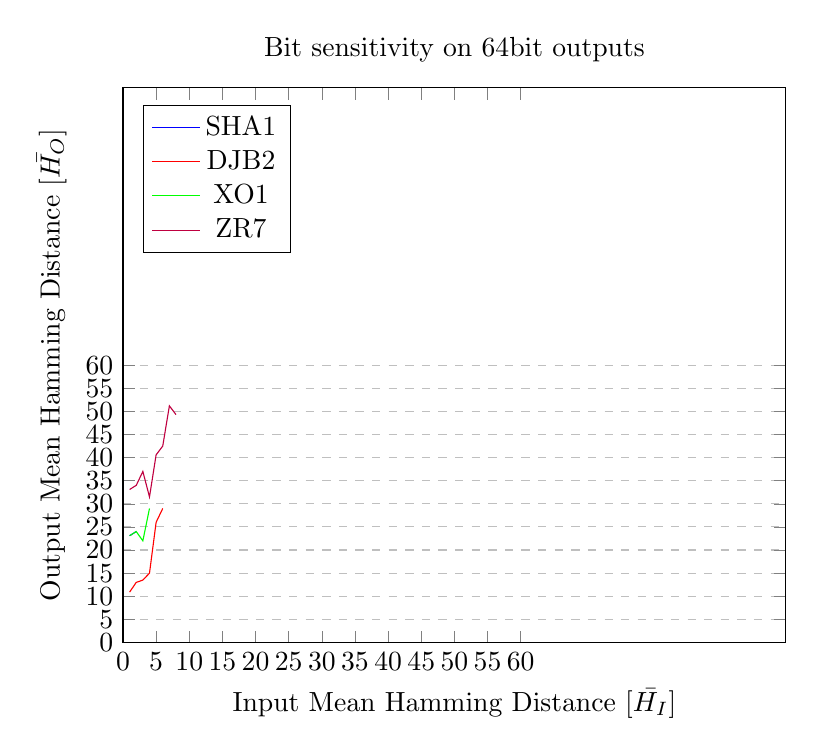
\begin{tikzpicture}
\begin{axis}[
    title={Bit sensitivity on 64bit outputs},
    xlabel={Input Mean Hamming Distance [$\Bar{H_I}$]},
    ylabel={Output Mean Hamming Distance [$\Bar{H_O}$]},
    xmin=0, xmax=100,
    ymin=0, ymax=120,
    xtick={0, 5, 10, 15, 20, 25, 30, 35, 40, 45, 50, 55, 60},
    ytick={0, 5, 10, 15, 20, 25, 30, 35, 40, 45, 50, 55, 60},
    legend pos=north west,
    ymajorgrids=true,
    grid style=dashed,
]

\addplot[
    color=blue
    ]
    coordinates {
    (1, 23.1)(2, 24)
    };
    \legend{ZR7}
    
\addplot[
    color=red
    ]
    coordinates {
    (1, 10.9)(2, 13)(3, 13.5)(4, 15)(5, 26)(6, 29)
    };
    \legend{DJB2}
    
\addplot[
    color=green
    ]
    coordinates {
    (1, 23.1)(2, 24)(3, 22)(4, 29)
    };
    \legend{XO1}
    
\addplot[
    color=purple
    ]
    coordinates {
    (1, 33.1)(2, 34)(3, 37)(4, 31.5)(5, 40.6)(6, 42.5)(7, 51.2)(8, 49.3)
    };
    \legend{SHA1, DJB2, XO1, ZR7}
    
\end{axis}
\end{tikzpicture}

\section{Discussion}

This is the results section

%\begin{tikzcd}
%A \arrow[rdd] \arrow[rd] \arrow[r, "\phi"] & B \\
%& C \\
%& D
%\end{tikzcd}

%\begin{figure}[h!]
%\centering
%includegraphics[scale=1.7]{universe}
%\caption{The Universe}
%\label{fig:universe}
%\end{figure}

\section{Conclusion}
This is the conclusion section

\bibliographystyle{plain}
\bibliography{references}
\end{document}
